\documentclass{standalone}
\usepackage{tikz}

\begin{document}
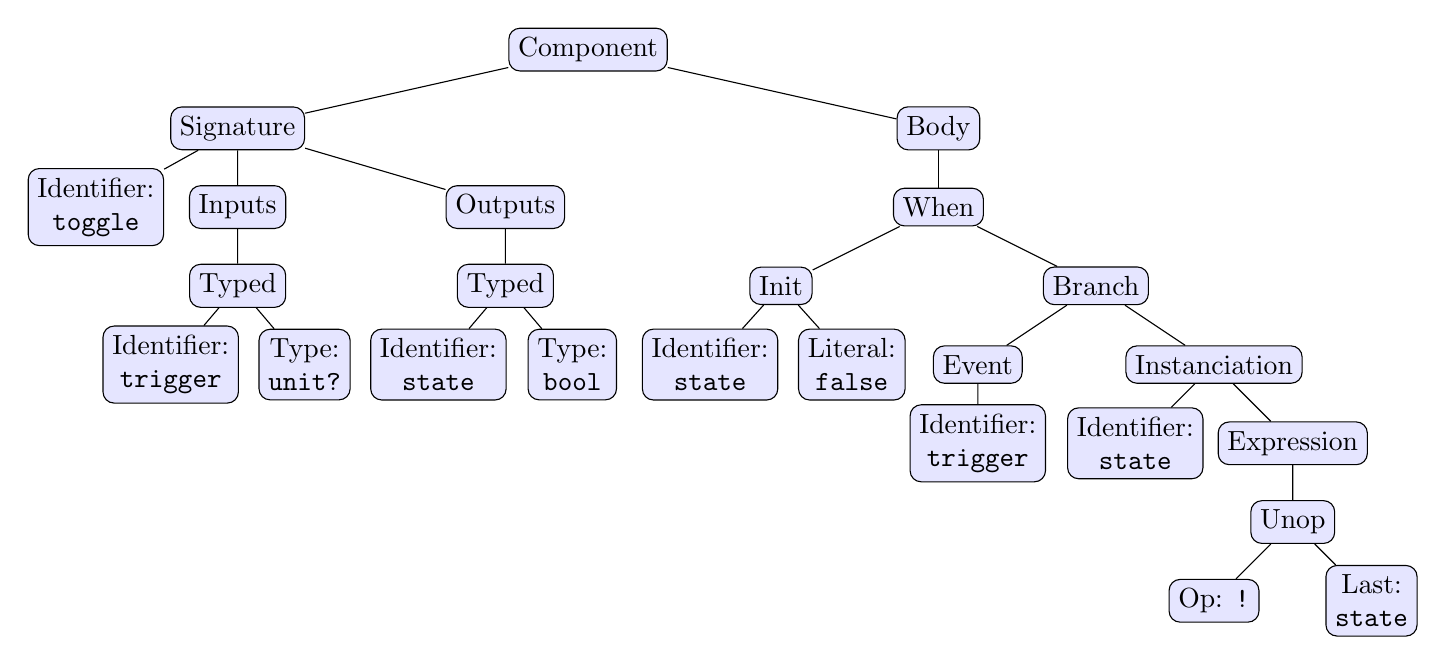
\begin{tikzpicture}[
                level distance=1cm, sibling distance=3cm,
                treenode/.style = {rectangle, rounded corners, draw, fill=blue!10, align=center}
        ]
        \node[treenode] {Component}
        child [sibling distance=8.9cm] { node[treenode] {Signature}
                        child [sibling distance=1.8cm] { node[treenode] {Identifier:\\\texttt{toggle}} }
                        child [sibling distance=3.4cm] { node[treenode] {Inputs}
                                        child [sibling distance=1.7cm] { node[treenode] {Typed}
                                                        child { node[treenode] {Identifier:\\\texttt{trigger}} }
                                                        child { node[treenode] {Type:\\\texttt{unit?}} }
                                                }
                                }
                        child [sibling distance=3.4cm] { node[treenode] {Outputs}
                                        child [sibling distance=1.7cm] { node[treenode] {Typed}
                                                        child { node[treenode] {Identifier:\\\texttt{state}} }
                                                        child { node[treenode] {Type:\\\texttt{bool}} }
                                                }
                                }
                }
        child [sibling distance=8.9cm] { node[treenode] {Body}
                        child { node[treenode] {When}
                                        child [sibling distance=4cm] { node[treenode] {Init}
                                                        child [sibling distance=1.8cm] { node[treenode] {Identifier:\\\texttt{state}} }
                                                        child [sibling distance=1.8cm] { node[treenode] {Literal:\\\texttt{false}} }
                                                }
                                        child [sibling distance=4cm] { node[treenode] {Branch}
                                                        child [sibling distance=3cm] { node[treenode] {Event} child { node[treenode] {Identifier:\\\texttt{trigger}} } }
                                                        child [sibling distance=3cm] { node[treenode] {Instanciation}
                                                                        child [sibling distance=2cm] { node[treenode] {Identifier:\\\texttt{state}} }
                                                                        child [sibling distance=2cm] { node[treenode] {Expression}
                                                                                        child { node[treenode] {Unop}
                                                                                                        child { node[treenode] {Op: \texttt{!}} }
                                                                                                        child { node[treenode] {Last:\\\texttt{state}} }
                                                                                                }
                                                                                }
                                                                }
                                                }
                                }
                };
\end{tikzpicture}
\end{document}
